\documentclass[11pt,twoside,a4paper]{article}
\usepackage{a4wide,amsmath,amssymb, amsthm}
\usepackage[english]{babel}		%add german if you want to write in German
\usepackage{graphicx}
\usepackage[T1]{fontenc}
\usepackage[hidelinks]{hyperref}


% If you want to use Umlaute (in German e.g. ä, ö, ü) directly instead of writing \"a, \"o, \"u
% then you can use either of the following options
%\usepackage[latin1]{inputenc}
%\usepackage{umlaut}


% If you want to customize the hypthenation of some words, you can add these (one by one) as follows
\hyphenation{hy-phen-ation}


%-------------------------- Formatting/Layout --------------------------%

% Adapting the layout, font etc. of captions:
% number is printed bold, font size is set to small
\usepackage[bf,small]{caption}
\usepackage{subcaption}
\usepackage{mathpazo}  % -- Palatino as font -- if this is not installed, simply comment this out
%\usepackage{mathptmx}  % -- Times as font 

% To differentiate between drafts and the final version you can use the following commands
%\usepackage{draftcopy}
%\draftcopySetGrey{0.90}   %   90% = very, very light grey
%\draftcopyName{DRAFT}{155}   % set any name you want
%\draftcopySetScale{1}

%--------------- Line- and indentations for paragraphs ----------------------%
\setlength{\parindent}{0em}
\setlength{\parskip}{\medskipamount}    % Space between paragraphs

% ---------- Environments for mathematical lemma, notations, remarks, examples etc. add more at your wish --------------------%
\newtheorem{theorem}{Theorem}
\newtheorem{notation}{Notation}
\newtheorem{defi}{Definition}
\newtheorem{kons}{Konstruktion}
\newtheorem{remark}{Remark}
\newtheorem{example}{Example}


% To provide the url command and to correctly handle URLs and e-mail adresses as \url{blabla@laberlaber.de}
\usepackage{url}

% --------------------- Own commands for numbers ---------%
\newcommand{\N}{\mathbb{N}}             % natural numbers
\newcommand{\Z}{\mathbb{Z}}             % integers
\newcommand{\R}{\mathbb{R}}             % reals



\begin{document}
\selectlanguage{english}	

\title{Advancing the Art of Internet Edge Outage Detection}
\author{Abhishek Shrestha \\
  (\texttt{abhishek.shrestha@campus.tu-berlin.de})\\[5mm]
  Seminar "Network Architectures: Internet Measurement'' , \\	%Please choose the right one
 Technische Universit{\"a}t Berlin
}
  
\date{SS\,2019}

\maketitle

% ---------------------------------------------------------------- INTRODUCTION -----------------------------------------------------------------------%
\section{Introduction}
 Internet connectivity has become ubiquitous in the modern society. Not only individual users but a multitude of critical services and business enterprises depend on a reliable network connection. Hence, over the years, a lot of resources and studies have been dedicated towards providing a more reliable service \hyperlink {K4}{[4 - 6]}. Among many other aspects, service availability is the most important measure of reliability. And judging the reliability of a network based on its availability should first involve understanding the cause, duration and frequency of failures across the network.
  
The authors in this paper present a prediction model to analyze and breakdown causes of internet disruptions and outages by studying the data from a large CDN and thereby try to provide a fine grain understanding of when and why these disruptions occur. 

Their study is based on the CDN access logs which contain entries of per hour requests sent by the connected address blocks. A sudden absence of entry in the log indicates a loss of internet connectivity in the specific IP address blocks, this is called a disruption. A service outage on the other hand means loss of internet access service in the address blocks. Therefore, although a disruption might be caused due to an actual service outage, every disruption does not necessarily mean that there was a service outage but instead a disruption might mean that the public IP of the host has changed or has been reassigned. Using the CDN log data as well as connectivity log from individual devices, collected over a selected duration, authors present a detailed study featuring size, timing and frequency of disruptions to argue that large share of detected disruptions or service outages might be due to planned human activities such as server maintenance and user mobility and thus might not always indicate network failures or issues. Another important aspect of the paper is that the authors, through the data, make a distinction between which disruptions represent an actual service outage and which are anti-disruptive events and not an actual service unavailability. Further, they compare their findings with Trinocular \hyperlink {K2}{[2]}, an established tool to measure internet outage to validate their results.

The rest of the paper is organized as follows: We discuss the related works in \hyperref[RW]{Section 2}. \hyperref[M]{Section 3} details the implemented methodology. \hyperref[RandEv]{Section 4} analyzes and interprets the results and also presents a comparison of results with Trinocular and finally \hyperref[DC]{Section 5} provides an overview of the work and discusses the implications of the work.

% -----------------------------------------------------------------RELATED WORK  --------------------------------------------------------------%
\section{Related Work}\label{RW}
There are a lot of research works in internet outage detection and reliability. Turner et al. \hyperlink {K3} {[3]} use router configuration files, syslog archives and operational mailing list to recreate failure events in a network. They then perform an extensive analysis of five years of such data from a network consisting of over two hundred routers. Basically, they extract the failure events from the syslog and router configuration files over the defined period and deduce cause of failure by referring to the administration email logs. The data is then analyzed for failure duration, cause and impact. One of the most significant features of their work is that the data sources used is easily available and is not restricted to a research group or require any special permission. Similarly, Banerjee \hyperlink {K1} {[1]} et al. use the outage mailing list \hyperlink{K17}{[17]} to investigate outages. The outage mailing list contains outage reports and discussion, impacts and troubleshooting information relating to major outages. This information is parsed using NLP and are then clustered into labeled categories using machine learning techniques and are then analyzed to derive probable cause, impact and type of disruption. The experiment was performed on outage data accumulated over seven years.

Benson et al. \hyperlink {K7} {[7]} use IBR traffic analysis to detect disruptions. Their methodology is rather interesting. Their system is based on observing IBR traffic from passive darknet \hyperlink {K8} {[8]}. IBR basically constitutes of TCP SYNs trying to connect to hosts but since darknet does not respond, these signals have to be retransmitted. These retransmissions follow a consistent pattern and thus the absence of these retransmission signals can be considered as packet loss and can be used to detect disruptions.

Trinocular \hyperlink {K2} {[2]} an outage detection system, uses active probing to detect disruptions. It sends multiple ICMP probes per hour to over 3 million /24 address blocks. If it detects any unresponsive prefixes, it flags it as a disruption. The authors compare their system against the disruptions detected by Trinocular.

% ---------------------------------------------------------------------- METHODOLOGY  ----------------------------------------------------------%
\section{Methodology}  \label{M}
This section describes in detail the dataset and the analysis methodology implemented by the authors.

%DATASET
\subsection{Dataset}
Each request from the client to access web object from CDN is logged. The authors used these CDN logs as the data set for analysis. The data set consists of number of hits or requests from each IP address for a period of 54 weeks (March 2017 - March 2018). The dataset is quite large (about 1.2 billion active IPv4 addresses over the course of one year),  considering they used logs from one of the world's largest CDNs which contained over 240,000 servers in over 13 countries and containing about 1,700 networks.

Due to hourly binning of datasets, for disruptions to be detected, they must last over a full calendar hour. CDN servers are generally in the same network as end user and also if there are any problems in connection to a server, as long as client has internet connection, user can be connected to another server and this usually takes less than a minute. So absence of hits from a particular IP address for about an hour indicates that either the device is disconnected by the client, loss of connection due to maintenance or could be due to other external events. 

%BASE LINE ACTIVITY
\subsection{Baseline activity as reference}
Always-on devices like mobile phones which are constantly connected to the network and make regular CDN requests provide us with a steady number of requests to CDN. This effect is called the baseline activity. The sudden absence of the requests from these devices can be recognized as a disruption. 

The authors selected a subset of prefixes which demonstrated this base line activity and limited their observation to only those prefixes which have a constant high enough baseline i.e. prefixes with sufficient number of addresses which show the base line activity. 
%fig 1a  and 1b here

\begin{figure}[h!]
  \centering
  \begin{subfigure}[b]{0.4\linewidth}
    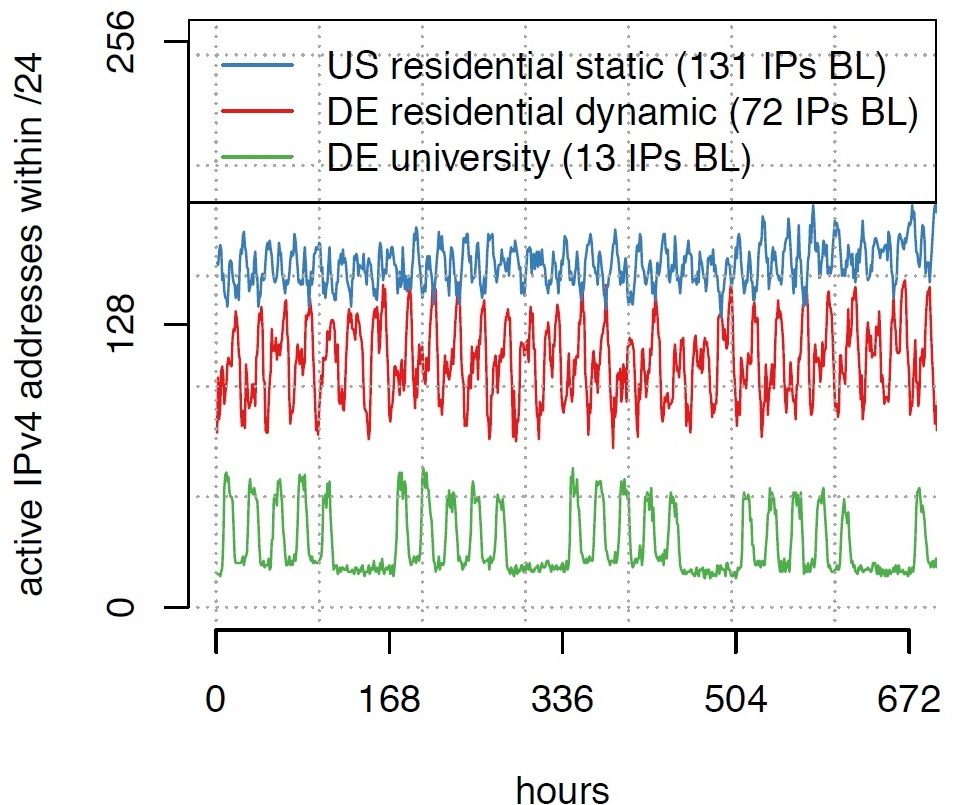
\includegraphics[width=\linewidth]{Figures/1a.png}
    \caption{Number of active addresses per hour studied for three /24 address blocks.}
  \end{subfigure}
  \begin{subfigure}[b]{0.4\linewidth} \hspace{6mm}
    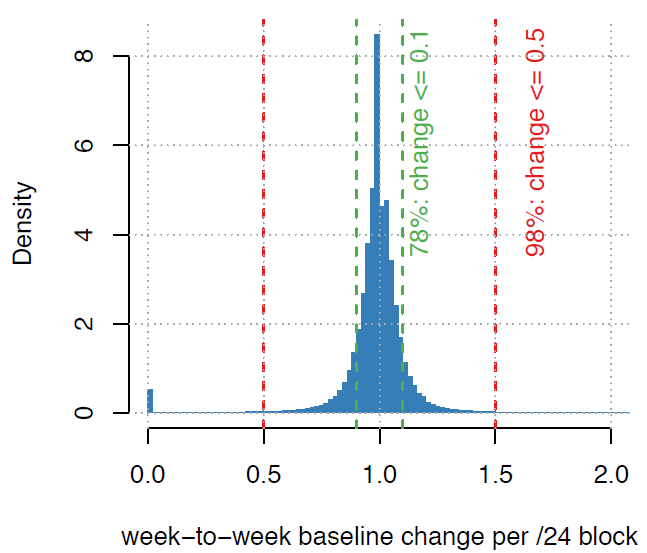
\includegraphics[width=\linewidth]{Figures/1c.png}
    \caption{Change in baseline activity in consecutive weeks.}
  \end{subfigure}
  \caption{Baseline activity illustration and behaviour.}
  \label{fig:BaselineDef}
\end{figure}

Figure 1a shows an example of baseline activity. The figure illustrates the number of active addresses per hour for three /24 address blocks for the duration of 3 months. As we can see all of these address blocks show a baseline activity i.e. over the duration of a month, each address block has a steady minimum number of devices connected for any given hour. The drop to minimum value during the end of the week for university address blocks is understandable since there are less number of students in the University during the weekends and hence less number of connected devices

For the purpose of evaluation throughout the year, the baseline activity should show a continuity i.e. the baseline should be maintained throughout the months over a whole year. Figure 1b shows that over 80\% of address block show only about 10\% change in baseline activity and only 2\% address blocks have baseline varying more than 50\%. To get the plot, for each /24 first, only those weeks which have minimum baseline of 40 were selected. Then the baseline of the week was divided by the baseline activity of the subsequent week where the subsequent week might have a baseline value greater or less than 40. Thus, we can see from the figure that the baseline activity is quite continuous.

% DETECTING DISRUPTION
\subsection{Detecting the disruptions}
For detecting the disruption a sliding window is used. For each /24, a minimum number of active addresses in each hour is calculated over the last 168 hours, this is denoted by $b_0$. Then the window is slid over an hour, updating the value of $b_0$. As soon as $b_0$ falls below a threshold $\alpha \times$ $b_0$ where 0 < $ \alpha$ < 1, the current window is left and a new window is created beginning at this hour and this hour is marked as the beginning of a non-steady-state period. The new window is slid and minimum value of $b_0$ is computed until it reaches a new threshold $\beta$ $\times$ $b_0$ where $\beta$ $\times$ $b_0$ is close to $b_0$ and this hour is then marked as the end of non-steady-state period. The non-steady-state period marks a disruption. This is illustrated in figure 2 for a single /24 address block.
%fig 2 here

\begin{figure}[h!] 
\centering
  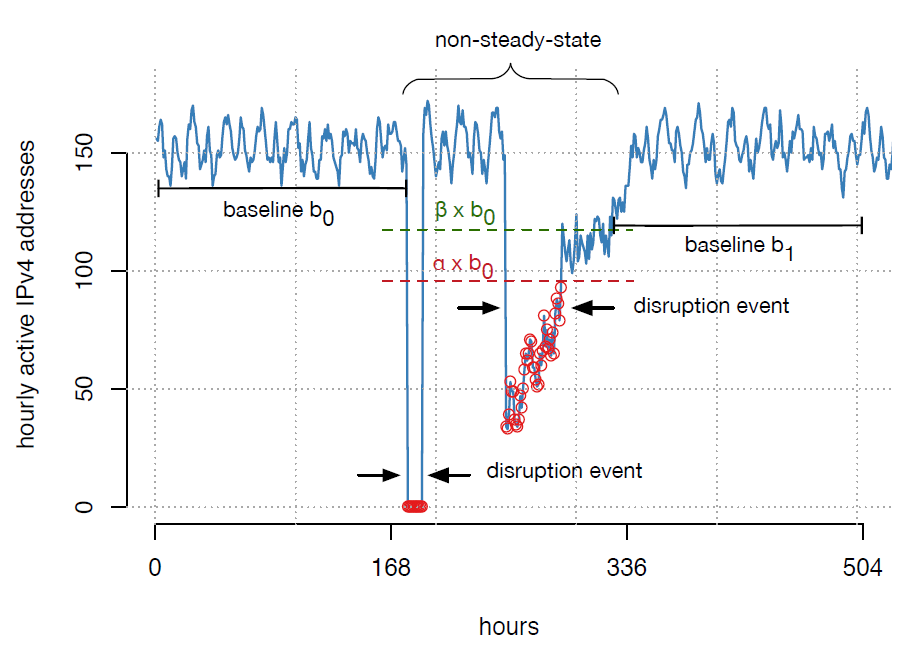
\includegraphics[width=0.6\linewidth]{Figures/2.png}
  \caption{Disruption detection using a sliding window of a fixed duration.}
  \label{fig:DisruptionDec}
\end{figure}

However, there is a possibility that after entering a non steady state period, the new base line $\beta \times b_0$ is never reached. The window is slid regardless, searching for the new baseline for 2 weeks. And if after 2 weeks the base line is not met then the non-steady-state is not regarded as disruption and the window is continued to slide.

% PARAMETER SELECTION
\subsection{Parameter selection}
Authors state in the paper that they performed several experimentations for the minimum value of $b_0$ and found that for a prefix to be traceable, the minimum number of active addresses should be at least 40.

A proper calibration of the values of $\alpha$ and $\beta$ is required for the algorithm to give accurate measurement. $\alpha$ being very low means that the algorithm will be less responsive while a high value of $\alpha$ would mean that the algorithm will be very sensitive to even slightest change in the baseline. Similarly, a high value of $\beta$ would mean that for a non-steady-state to be classified as disruption, baseline has to be restored to values closer to $b_0$, while low value of $b_0$ would mean that it will take less addresses to be active again for a non-steady-state to be classified as a disruption, and hence there is possibility that long term baseline changes might be considered as a disruption.

For determining proper values of $\alpha$ and $\beta$, disruptions detected against various values of $\alpha$ and $\beta$ are compared against ICMP probing responsiveness. We can see from figure 3a that a disruption i.e. loss of activity in CDN is also accompanied by a distinct drop in ICMP responsiveness. We can use this metric to calibrate proper values for $\alpha$ and $\beta$.
%fig 3a and 3b here
\begin{figure}[h!]
  
  \begin{subfigure}[b]{80mm}
    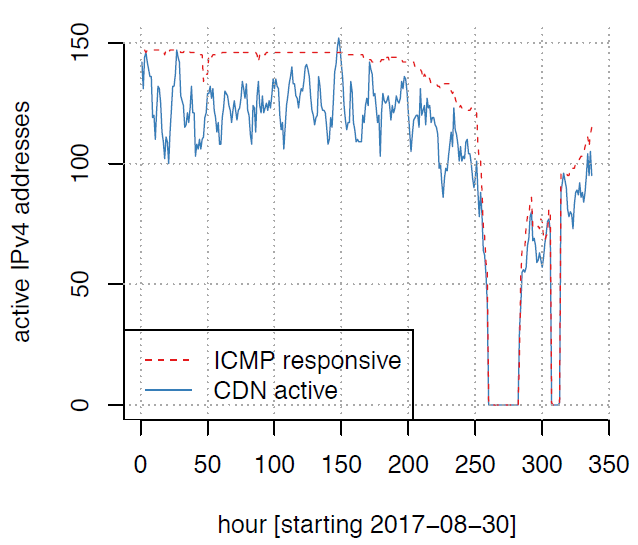
\includegraphics[width=\linewidth]{Figures/3a.png}
    \caption{A drop in CDN activity accompanied by a drop in ICMP responsiveness.\newline\newline}
  \end{subfigure}
  \begin{subfigure}[b]{75mm}  \hspace{5mm}
    {\raisebox{1mm}{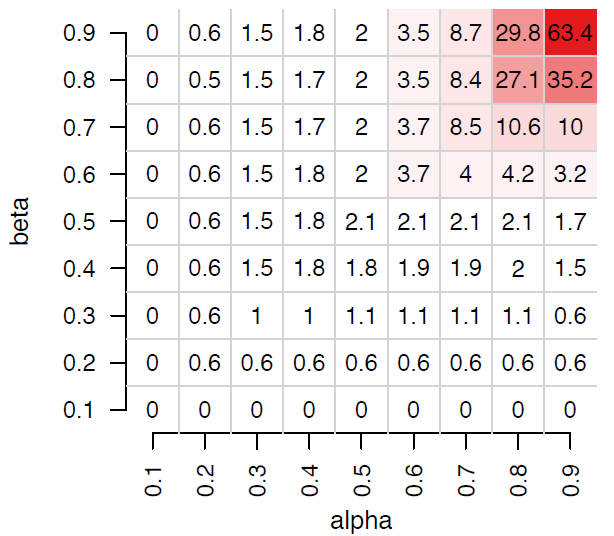
\includegraphics[width=\linewidth]{Figures/3b.png}}}
    \caption{Percentage disagreement between CDN and ICMP for different combination of values of $\alpha$ and $\beta$. \newline}
  \end{subfigure}
  \caption{Coorelation between ICMP responsiveness and CDN activity.}
  \label{fig:CDNAndICMP}
\end{figure}

Since actively probing a large address space requires substantial bandwidth and also according to authors, about 40\% of addresses contacting CDN do not respond to ICMP probes. Therefore, they used already available ICMP data from ISI \hyperlink {K9} {[9 -12]}. The data is from four surveys between June and September 2017. Since, comparison is done against CDN data, the addresses in the survey data must also overlap with CDN. So, all addresses that are not in CDN are removed and also the address blocks that have less than 40 responsive addresses are removed which resulted in about 15K ISI data for comparison.  

Authors then selected various combinations of values of $\alpha$ and $\beta$. Then the non-steady-states detected by each combination are compared against the ISI dataset. And as mentioned earlier the disruptions must also show a drop in ICMP responsiveness and for those which are not classified as disruptions, the ICMP responsiveness should not drop below 40. If the maximum value of ICMP responsive address during the disruption is less than the minimum value outside the disruption, then the disruption is classified as "agree" otherwise it is classified as  "disagree".

Figure 3b shows percentage of disagreement of CDN detection with the ISI data for different values of $\alpha$ and $\beta$. As we can see, for very low values of $\alpha$ and $\beta$ the disagreement is also very low. This makes sense since low values of $\alpha$ and $\beta$ means that the algorithm is more restrictive, for instance, if we consider $\alpha$ as 0.1 then this would require the active addresses to drop significantly (near 0) to be classified as disruption. This would definitely also be accompanied by drop in ICMP responsiveness because of drastic drop in active addresses. In contrast, for high values of $\alpha$ and $\beta$ the disagreement is also higher. This is also obvious since high values of $\alpha$ and $\beta$ would make the algorithm more sensitive. Authors end up selecting $\beta$ as 0.8, since a higher value of $\beta$ means that the system would want more addresses to be active to consider a period to be classified as a disruption. This makes the system more restrictive and removes possibility of considering slight increase in active addresses to be end of a non-steady-state period. Moreover, for smaller values of $\alpha$, $\beta$ does not increase considerably for any value. Higher value of $\beta$ is therefore more appropriate.  Considering $\beta$ as 0.8, from figure 3b we can see that the disagreement increases in large steps after $\alpha$ is greater than 0.5. Thus, from this observation, $\alpha$ is then fixed at 0.5 to keep the disruption under 3\%.

% ---------------------------------------------------------------------- RESULTS AND EVALUATION  ----------------------------------------------------------%
\section{Results and evaluation} \label{RandEv}
% OUTCOMES AND EXPERIMENTS
\subsection{Outcomes and experiments}
%fig 4 here.

\begin{figure}[h!] 
\centering
  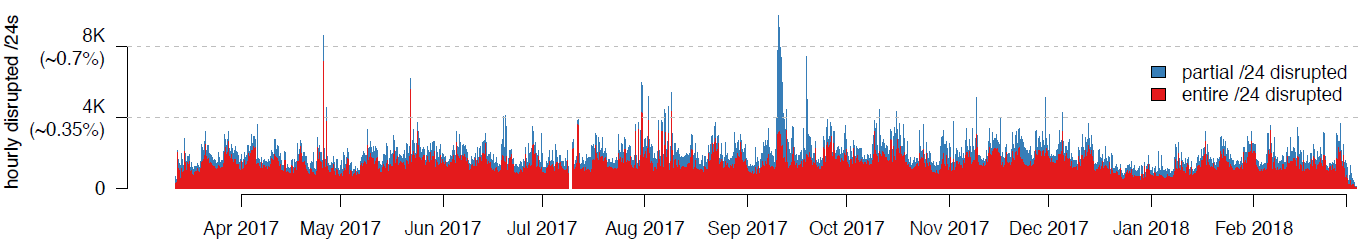
\includegraphics[width=\linewidth]{Figures/4.png}
  \caption{Number of disrupted address blocks per hour during the full year study period (March 2017 to March 2018)}
  \label{fig:Result}
\end{figure}
Once the parameters are established, the authors applied the algorithm over the entire study period. Figure 4 shows the number of disrupted /24 address blocks in each hour from March 2017 to March 2018. The red bars in the figure show that for the duration the active addresses for the /24 block went down to 0 while blue indicates that some addresses were still active during the disruption.

We can observe from the figure that during September there was a huge disruption where more than 8k addresses went down. This coincides with the hurricane Irma. So the sudden spike is due to a natural disaster.

From the figure we can see somewhat uniform disruption pattern over the weeks. Figure 5a shows the disruptions per day for an isolated week. We can see that the disruptions are higher during Tuesday, Wednesday and Thursday, which is a typical server maintenance window. This becomes clearer when referring to figure 5b. As shown in the figure the disruptions usually happen between 1 A.M. and 3 A.M, which is the maintenance time for most of the servers. This emphasizes that most of the disruption events during the week can be credited to planned maintenances. 

%fig 5 a. and 5 b. here
\begin{figure}[h!]
  \centering
  \begin{subfigure}[b]{0.47\linewidth}
    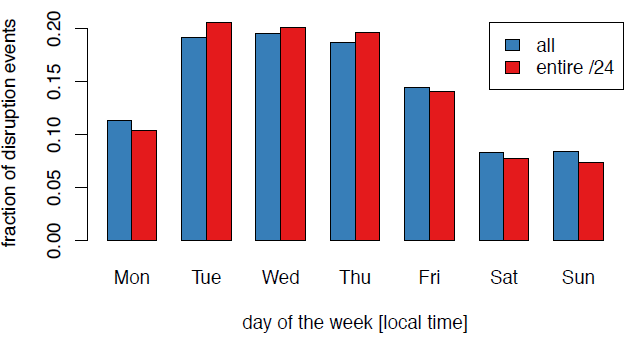
\includegraphics[width=\linewidth]{Figures/5a.png}
    \caption{Disruption pattern viewed per day over a week.}
  \end{subfigure}
  \begin{subfigure}[b]{0.47\linewidth}
    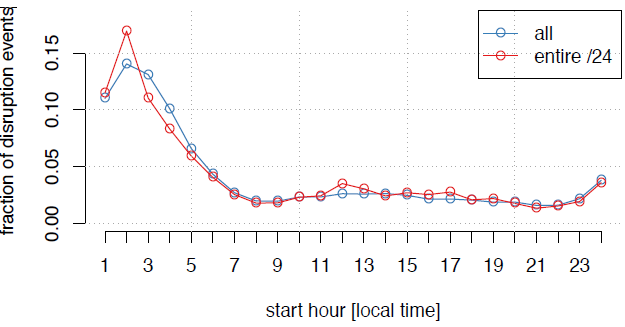
\includegraphics[width=\linewidth]{Figures/5b.png}
    \caption{Start hour of disruption viewed over 24 hours of a day}
  \end{subfigure}
  \caption{Analyzing time of disruption by viewing disruption patterns over a single week and a single day.}
  \label{fig:coffee}
\end{figure}

For further analysis of the disruption events and to actually understand whether or not these were actual service outages, the connectivity of individual devices to CDN during the disruptions was analyzed. For this, the individual device activity before, during and after the disruptions had to be tracked. Tracking the activity of individual device was made possible by a software which clients could voluntarily install in their devices. The software supported both Windows and Mac OS X but could only run on desktops and laptops but not on smart phones.  

This software makes repeated pings to CDN. Each software installation associates the device with a unique software ID and every time the device contacts the CDN, the time stamp along with this ID and the device IP at the time is logged. This log is different from the CDN log as this log only includes those devices that installed the software and contains an ID which identifies a unique device. Now, this log can be cross referenced with the CDN log to see whether the device was actually active or not during the disruption.

%fig 6 here
\begin{figure}[h!] 
\centering
  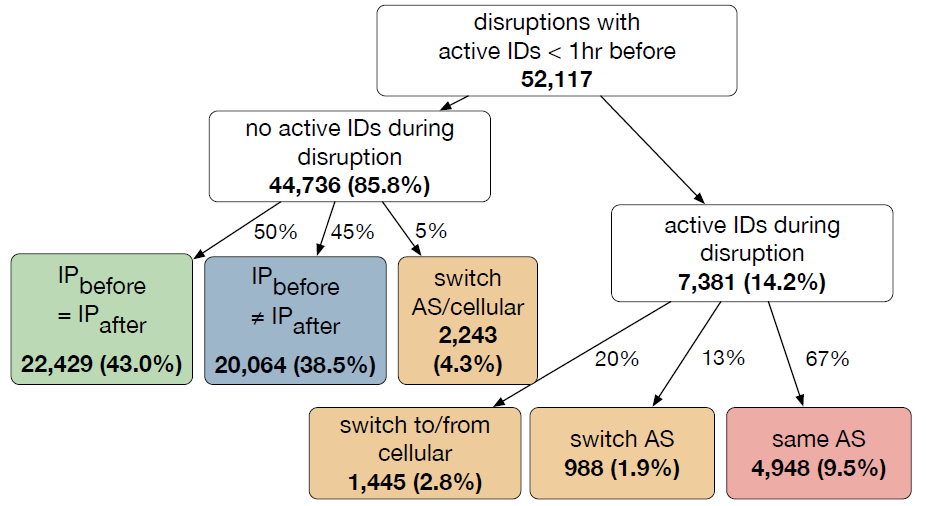
\includegraphics[width=0.6\linewidth]{Figures/6.png}
  \caption{Device's connectivity verified by cross-referencing CDN logs with software ID logs.}
  \label{fig:DeviceIDLog}
\end{figure}
For the purpose of this study, authors considered only those /24 address blocks which were entirely affected by disruption (active addresses went 0). These addresses can then be checked using the log obtained from devices to see if the device was active during the disruption in different address block. Figure 6 shows the result of these comparisons. In the figure, $IP_{before}$ means the IP of the device before the disruption, $IP_{after}$ means the IP of the device after the disruption and $IP_{during}$ means the IP of the address during the disruption.

About 14\% of the devices showed activity even during the disruptions (in different address block). Authors assume that this could be attributed to various reasons like the user could have moved to some different location or connected their device to a different network. Another reason, they explain, could be that the IP address with which the user is connected was changed, thus causing sudden absence of activity in the initial address block and abrupt increase of activity in alternate address block in the same AS. This phenomenon is termed as "anti-disruption". These anti-disruptive events account for about 10\% of the disruptions. After contacting several ISPs authors were able to confirm that majority of ISPs do indeed reassign prefixes and some do so more frequently. If one were to assume all disruptions are service outages then these anti-disruptive events can cause a network to seem to have bad reliability.   
Now, considering those devices that did not show activity during the disruption (about 86\%), 43\% of these devices had the same IP before and after the disruption. Authors believe that it is unlikely that the devices were assigned a new IP temporarily and again were reverted back to the original IP so this indicates an actual service outage. However, for the cases when the IP before the disruption is different that the IP after the disruption, there is an ambiguity about the cause as this could be due to actual outage, address reassignment or device movement.

% EVALUATION AGAINST TRINOCULAR
\subsection{Evaluation against Trinocular} 
The authors compared the disruptions detected by their algorithm against those detected by Trinocular, which is another disruption detection system. They used a three month (April 2017 - July 2017) ISI dataset \hyperlink {K13}{[13]} to implement Trinocular. They then evaluated the visibility of disruptions detected by their algorithm in Trinocular detected disruptions and vice versa. 

For comparing the disruption detected by Trinocular with the CDN detected disruptions, only those disruptions in the Trinocular dataset that lasted more than an hour were filtered. About 29.9\% of the disruptions in the Trinocular dataset lasted more than an hour. The authors found out that Trinocular detected significantly more disruptions than the disruptions detected from the CDN logs. Only about 27\% of the disruptions detected by Trinocular agreed with the disruptions detected by the CDN logs. About 13\% of the disruptions detected by Trinocular were reflected in terms of reduced CDN activity in the CDN logs but these were not below the threshold to be detected as disruptions. For about 60\% of the disruptions in Trinocular, the CDN activity was normal, indicating that Trinocular was detecting more disruptions than actual occurrences.

To find the cause this discrepancy, the authors communicated with the developers of Trinocular and confirmed that Trinocular does detect false positives and it is a known issue with their system. Therefore, authors further narrowed down the data set by considering only address blocks with less than 5 disruptions, decreasing the number of disruptions for comparison to 110K. After filtering, 74\% percent of the disruptions detected by Trinocular agreed with the CDN detected disruptions.

Next, authors compared the CDN detected disruptions with the Trinocular detected disruptions. For this, only the disruptions in CDN that affected the whole /24 blocks were considered since Trinocular detects disruptions in block-level. About 94\% of the disruptions detected by Trinocular agreed with the CDN detected disruptions in this case. The authors then applied the same filter as before and found out that after filtering only 74\% of the disruptions were agreeable. Thus, although filtering increased the visibility of Trinocular detected disruption in CDN detected disruptions by 47\%, it also decreased the visibility of CDN detected disruption in Trinocular by 20\%.

% ---------------------------------------------------------------------- DISCUSSION AND CONCLUSION ----------------------------------------------------------%
\section{Discussion and conclusion} \label{DC}
The authors, in their paper offer a passive approach in detecting internet outages and disruptions. Their detailed analysis of the results and experiments offer a clearer picture of probable causes and in-depth interpretation of disruptions. Their findings suggest that in majority of cases, the outages can be attributed to planned human activities. And a disruption does not necessary mean loss of network connectivity or an outage but can be due to service providers re-assigning IP addresses.

The authors, while cross validating the device IDs and IP addresses obtained from the device activity log with the CDN logs found that there were less than 0.01\% devices which were seen to be active and have IP addresses during the disruption in the disrupted blocks. This is a very low error margin and implies that their algorithm is accurate enough. Using the device activity log, they also found out that about 10\% of the disruptions were caused due to anti-disruption events. These anti-disruptions can potentially cause a network to seem to have less reliability.

Although the methodology and the findings are significant, it is not without its flaws. One of the flaws with their approach is that they use proprietary data which is not universally available. This severely imposes limits on anyone or any groups trying to extend or build on in their work. Another flaw is that the device ID log does not include smart phones whereas smart phones may have contributed heavily to the baseline activity in the CDN logs. So it seems that the results obtained from cross referencing these logs to confirm whether the devices were actually online during disruptions seems to be quite unreliable.   

\textbf{Future Work:} From small business using the internet connectivity for growth \hyperlink {K14} {[14]} to large cities implementing ideas like IOT for better sustainability, efficiency and citizen welfare \hyperlink {K15} {[15-16]}, the number of applications and services which need internet for functionality are growing. Internet is becoming a requirement rather than a luxury and thus proper understanding and interpretation of internet outages is important and will become more crucial in the coming days. Thus, there are bound to be more studies and research work in this area. Fortunately, since the devices and services that connect to internet are growing, they are also providing more data and this provides more opportunities to perform more detailed and accurate studies on outages.


\begin{thebibliography}{12}

        
\bibitem[1]{1} \hypertarget{K1} 
       R. Banerjee, A. Razaghpanah, L. Chiang, A. Mishra, V. Sekar, Y. Choi, and P. Gill: {\sl Internet Outages, the Eyewitness Accounts: Analysis of the Outages Mailing List}. 
       Passive and Active Measurement (PAM), Mar 2015, S. 206-219.
        
\bibitem[2]{2} \hypertarget{K2} 
       L. Quan, J. Heidemann, and Y. Pradkin: {\sl Trinocular: Understanding Internet Reliability Through Adaptive Probing}. 
       ACM SIGCOMM, Aug 2013, S. 255-266.
       
\bibitem[3]{3} \hypertarget{K3} 
       D. Turner, K. Levchenko, A. C. Snoeren, and S. Savage: {\sl California Fault Lines: Understanding the Causes and Impact of Network Failures}. 
       ACM SIGCOMM, 2010, S 315-326.
              
\bibitem[4]{4} \hypertarget{K4} 
         Morton E O'Kelly, Hyun Kim, Changjoo Kim: {\sl Internet Reliability with Realistic Peering.}. 
         Environment and Planning B: Planning and Design, 33(3), 2006, S 325-343.
     
\bibitem[5]{5} \hypertarget{K5} 
        A.K.Y. Wong ; T.S. Dillon: {\sl A fault-tolerant data communication setup to improve reliability and performance for Internet based distributed applications}. 
       Proceedings 1999 Pacific Rim International Symposium on Dependable Computing, 1999, S 268-275.
                
\bibitem[6]{6} \hypertarget{K6} 
         FCC. 
          {\sl CFR Part 4 -DISRUPTIONS TO COMMUNICATIONS. Outage reporting requirements - threshold criteria.}. 
         \href{https://www.law.cornell.edu/cfr/text/47/part-4}{https://www.law.cornell.edu/cfr/text/47/part-4}
       
\bibitem[7]{7} \hypertarget{K7} 
       K. Benson, A. Dainotti, KC Claffy, E. Aben: {\sl Gaining Insight into AS-level Outages through Analysis of Internet Background Radiation}. 
       ACM SIGCOMM Conference on emerging Networking EXperiments and Technologies (CoNEXT) Student Workshop, Dec 2012, S. 63-64.
       
\bibitem[8]{8} \hypertarget{K8} 
       R. Pang, V. Yegneswaran, P. Barford, V. Paxson, and L. Peterson: {\sl Characteristics of Internet Background Radiation}. 
       Internet Measurement Conference (IMC 2004), Oct 2004, S. 27-40.
       
 \bibitem[9]{9} \hypertarget{K9} 
        Internet Addresses Survey dataset. 
        {\sl PREDICT ID: USC-LANDER/internet-addresssurvey-reprobing-it76c-20170723/rev7956. Traces taken 2017-07-23 to 2017-08-06.Provided by the USC/LANDER project}. 
        \href{http://www.isi.edu/ant/lander}{http://www.isi.edu/ant/lander}
        
\bibitem[10]{10} \hypertarget{K10} 
        Internet Addresses Survey dataset. 
        {\sl PREDICT ID: USC-LANDER/internet-addresssurvey-reprobing-it76w-20170628/rev7942. Traces taken 2017-06-28 to 2017-07-13. Provided by the USC/LANDER project}. 
        \href{http://www.isi.edu/ant/lander}{http://www.isi.edu/ant/lander}
        
\bibitem[11]{11} \hypertarget{K11} 
        Internet Addresses Survey dataset. 
        {\sl PREDICT ID: USC-LANDER/internet-addresssurvey-reprobing-it77c-20170914/rev8018. Traces taken 2017-09-14 to 2017-09-29. Provided by the USC/LANDER project}. 
        \href{http://www.isi.edu/ant/lander}{http://www.isi.edu/ant/lander}

\bibitem[12]{12} \hypertarget{K12} 
        Internet Addresses Survey dataset. 
        {\sl PREDICT ID: USC-LANDER/internet-addresssurvey-reprobing-it77w-20170830/rev8013. Traces taken 2017-08-30 to 2017-09-14. Provided by the USC/LANDER project}. 
        \href{http://www.isi.edu/ant/lander}{http://www.isi.edu/ant/lander}
        
\bibitem[13]{13} \hypertarget{K13} 
        Internet Outage Dataset. 
        {\sl PREDICT ID: USC-LANDER/internet-outage-adaptivea28all-20170403. Provided by the USC/LANDER project}. 
        \href{http://www.isi.edu/ant/lander}{http://www.isi.edu/ant/lander}
        
\bibitem[14]{14} \hypertarget{K14} 
       B. M. Sadowski, C. F. Maitland, J. V. Dongen: {\sl Strategic use of the Internet by small- and medium-sized companies: an exploratory study}. 
       Information Economics and Policy, 14(1), Mar 2002, S. 75-93.

\bibitem[15]{15} \hypertarget{K15} 
       A.M Townsend: {\sl Network Cities and the Global Structure of the Internet}. 
       American Behavioral Scientist, 44(10), Jun 2001, S. 1697-1716. 
       
\bibitem[16]{16} \hypertarget{K16} 
       S. Alawadhi, A. Aldama-Nalda, H. Chourabi, J. Ramon Gil-Garcia, S. L. Mellouli, T. Nam, T. A. Pardo, H. J. Scholl, S. Walker: {\sl Building Understanding of Smart City Initiatives}. 
       Electronic Government (EGOV), 7443, 2012. S. 40-53.       

\bibitem[17]{17} \hypertarget{K17} 
        V. Rode: {\sl Outages - outages (planned \& unplanned) reporting}. 
        \href{https://puck.nether.net/mailman/listinfo/outages}{https://puck.nether.net/mailman/listinfo/outages}
       
\end{thebibliography}
\end{document}

